\documentclass[rep.tex]{subfiles}
\begin{document}

\chapter{Zadanie 5}
\label{zad5}
\section{Treść}
Wykorzystując oprogramowanie napisane do rozwiązania zadania~\ref{zad4} wyznaczyć impedancję charakterystyczną powietrznej linii TEM o przekroju poprzecznym jak na rys.~\ref{fig:zad5:line},
przyjmując $b = 8~mm$ i $t = 4~mm$.
Wynik otrzymany numerycznie porównać z wynikiem obliczonym według odpowiednich,
przybliżonych wzorów wykorzystujących całki eliptyczne.

\begin{figure}[!htbp]
  \centering
  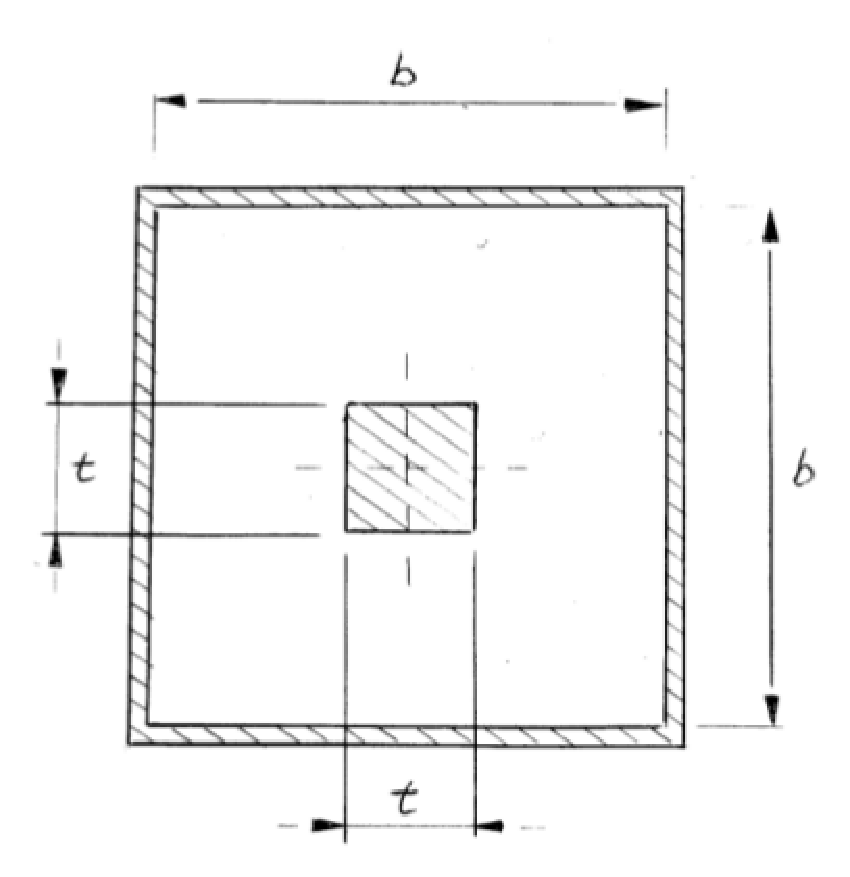
\includegraphics[scale=0.5]{fig/zad5/line}
  \caption{Linia rozważana w zadaniu~\ref{zad5}}
  \label{fig:zad5:line}
\end{figure}

\section{Rozwiązanie}
Impedancja linii została wyznaczona w sposób opisany w sekcji~\ref{zad4:thick}.
Dla linii określonej w niniejszym zadaniu wynosi ona~$Z_0 = 36.7605605644~\Omega$.

\begin{figure}[!htbp]
  \centering
  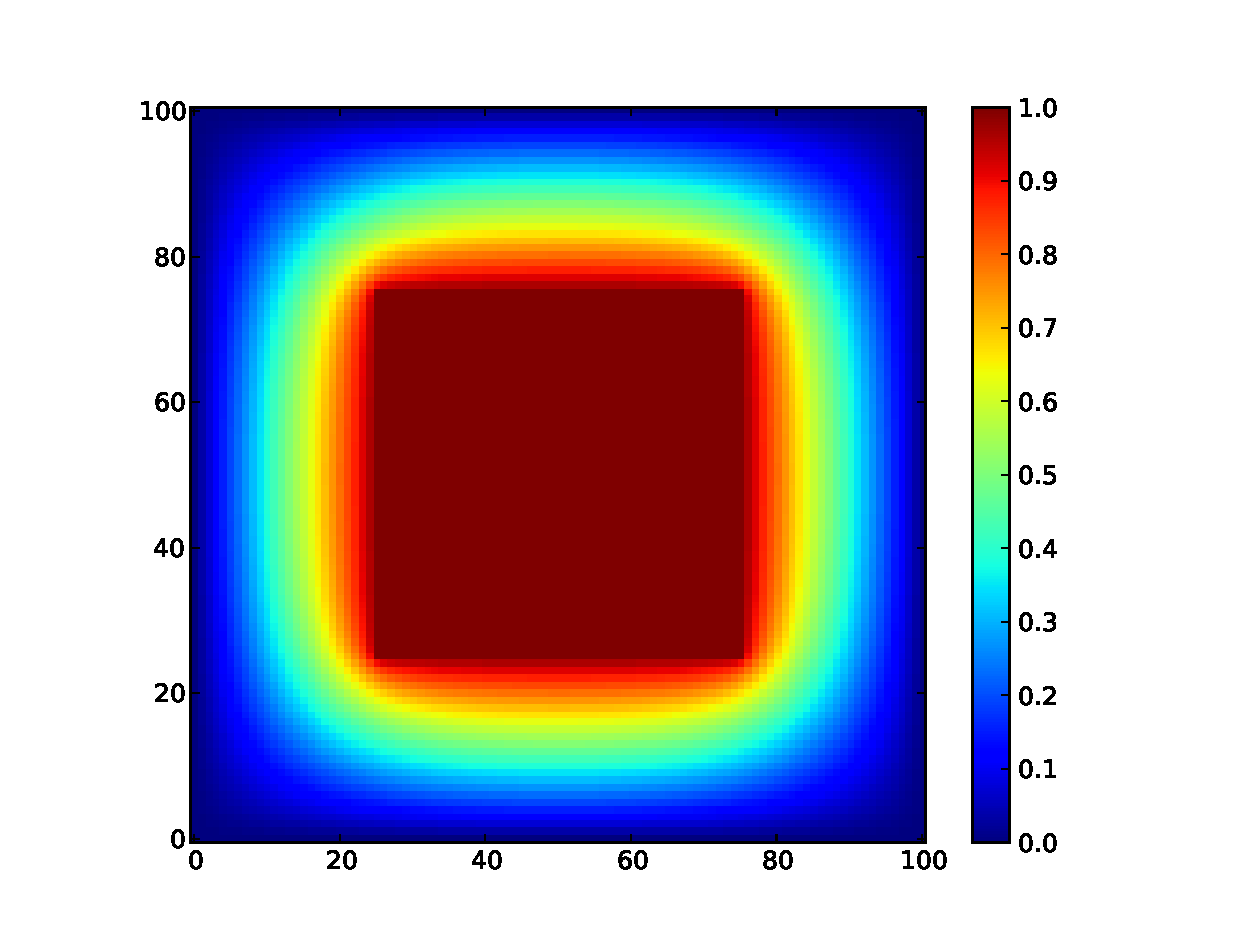
\includegraphics[scale=0.5]{fig/zad5/u}
  \caption{Rozkład potencjału w linii współosiowej z kwadratowymi przewodami}
  \label{fig:zad5:u}
\end{figure}

Impedancja obliczona według przybliżonego wzoru opartego o całki eliptyczne wynosi~$Z_0 = 36.807171466~\Omega$.
Jest to wynik bardzo bliski uzyskanemu za pomocą metody różnic skończonych.
\end{document}
